

%-------------------------------------------------------------------------------
% Dokumenten Klasse
\documentclass[
	final,
	a4paper,
	oneside,
	parskip=full,
	headings=standardclasses,
	headings=big,
	pointednumbers,
    fleqn
]{scrartcl}

%-------------------------------------------------------------------------------
% Packete nutzen
\usepackage{ngerman,palatino,setspace}
\usepackage[T1]{fontenc}
\usepackage[utf8]{inputenc}
\usepackage[left=20mm,right=20mm,top=10mm,bottom=25mm]{geometry}
\usepackage{amsmath}
\usepackage{amssymb}
\usepackage{mathtools}

%-------------------------------------------------------------------------------
\usepackage{xcolor}

%-------------------------------------------------------------------------------
% dbox
\usepackage{dashbox}

%-------------------------------------------------------------------------------
% uline
\usepackage{ulem}

%-------------------------------------------------------------------------------
% TikZ
\usepackage{tikz}
%\usetikzlibrary{positioning, arrows, decorations}
\usetikzlibrary{arrows,decorations.pathmorphing,backgrounds,positioning,fit,petri}

\tikzset{
    myptr/.style={
        ->,
        >=stealth
    }
}

%-------------------------------------------------------------------------------
% Für enumerate
\usepackage{enumitem}
\setlist[enumerate]{
    wide=0pt,
    leftmargin=*,
    itemsep=-1ex,
    parsep=2ex,
    labelsep=1ex,
    label=\alph*)
}

\usepackage{multirow}
\usepackage{ifthen}

%-------------------------------------------------------------------------------
% tabu
\usepackage{tabu} 

%-------------------------------------------------------------------------------
% table line breaks with \makecell
\usepackage{makecell}
\renewcommand\cellalign{bl}

%-------------------------------------------------------------------------------
% 
\usepackage{xparse}
% 1: Subscription  (default: '')
% 2: Funktion Name (default: 'f')
% 3: Argument      (default: 'x')
% \fx         = f(x)
% \fx[1]      = f_1(x)
% \fx[][u]    = u(x)
% \fx[][u][x] = u(x)
% \fx[][f][u] = f(u)
\NewDocumentCommand{\fx}{ O{} O{f} O{x} }{{#2_{#1}{\left( #3 \right)}}}
\NewDocumentCommand{\dfx}{ O{} O{f} O{x} }{{#2'_{#1}{\left( #3 \right)}}}
\NewDocumentCommand{\dx}{ O{} }{{\Delta x^{#1}}}
\NewDocumentCommand{\dy}{ O{} }{{\Delta y^{#1}}}
\NewDocumentCommand{\dt}{ O{} }{{\Delta t^{#1}}}
\NewDocumentCommand{\gp}{ O{} }{}


% 1: Funktion Name
% 2: dx
% 3: dx^2
% 4: x_1
% 5: x_2
% 5: x_3
\NewDocumentCommand{\gpp}{ O{} O{\dx} O{\dx[2]} O{x} O{x} O{x} }{%
    \frac{1}{#3}
    \kl{#1 
        \kl{#4 \ifthenelse{\equal{#2}{}}{}{+ #2}} - 
        2 \cdot #1\kl{#5} +
        #1 \kl{#6\ifthenelse{\equal{#2}{}}{}{- #2}}
    }
}

% 1: x_1
% 2: x_2
% 3: x_3
% 4: dx^2
\NewDocumentCommand{\gppn}{ O{x_1} O{x_2} O{x_3} O{?}}{%
    \frac{1}{#4}
    \kl{#1 - 2 \cdot #2 + #3}
}

\newcommand{\f}[2]{\frac{#1}{#2}}
\newcommand{\e}{\mathrm{e}}
\newcommand{\kl}[1]{{\left( #1 \right)}}
\newcommand{\kq}[1]{{\left\{ #1 \right\}}}
\newcommand{\ks}[1]{{\left[ #1 \right]}}

%-------------------------------------------------------------------------------
% Dokument
\begin{document}

    \subsection*{Ableitungsregeln}
    
    \renewcommand{\arraystretch}{1.25}
    \begin{tabular}{lll}
        Faktorregel  & $ y = C \cdot \fx$                   & $ y' = C \cdot \dfx $ \\
                     & $ y = 5 \cdot x^2 $                  & $ y' = 5 \cdot 2 \cdot x$ \\
        Summenregel  & $ y = \fx[1] + \ldots +  \fx[n] $    & $ y' = \dfx[1] + \ldots + \dfx[n] $\\
                     & $ y = x^2 + x^3$                     & $ y' = 2 \cdot x + 3 \cdot x^2$ \\
        Produktregel & $ y = \fx[][u] \cdot \fx[][v] $      & $ y' = \fx[][u] \cdot \dfx[][v] + \dfx[][u] \cdot \fx[][v] $ \\
                     & $ y = x^2 \cdot e^{2x}  $            & $ y' = x^2 \cdot 2\cdot e^{2x} + 2\cdot x \cdot e^{2x} $ \\
                     &                                      & $ y' = {\left( 2x^2 + 2x \right)} e^{2x} $ \\
        Kettenregel  & $ y = f\kl{u\kl{x}} $                & $ y' = \dfx[][f][u] \cdot \dfx[][u][x] $ \\
                     & $ y = f\kl{x^2 - 5}, \; f = x^2 $    & $ y' = 2 u \cdot 2x = 4x \kl{x^2 - 5} $ \\
                     & $ y = \ln\kl{1 + x^2} $              & $ y' = \frac{1}{u} \cdot 2x = \frac{2x}{1 + x^2} $ \\
    \end{tabular} \\

    {\renewcommand{\arraystretch}{1.75}
    \begin{tabular}{ll}
        Forward FDM  & $g'\kl{x} = \frac{g \kl{x + \dx} - g \kl{x}}{\dx}$ \\
        Backward FDM & $g'\kl{x} = \frac{g \kl{x} - g \kl{x - \dx}}{\dx}$ \\
        Central FDM  & $g'\kl{x} = \frac{g \kl{x + \dx} - g \kl{x - \dx}}{\dx}$
    \end{tabular}}
    
    \begin{align*}
        g'\kl{x}  &= \frac{g \kl{x + \dx} - g \kl{x}}{\dx} \\
        g''\kl{x} &= \frac{g \kl{x + \dx} - 2 \cdot g\kl{x} + g \kl{x - \dx}}{\dx[2]}
    \end{align*}


    Stationary Temperature Profile $T\kl{x}$ in a long, slim, not isolated rod of length $L$:
    \begin{align*}
        \SwapAboveDisplaySkip
        T''\kl{x} + h \cdot \kl{T_A - T\kl{x}} = 0, \qquad T\kl{0} = T_0, \quad T\kl{L}=T_L & &
    \end{align*}
    Concrete values:
    \begin{align*}
        \SwapAboveDisplaySkip
        L = 10\mathrm{m} \quad
        h = 0.01 {\textstyle \frac{1}{\mathrm{cm}^2}} \quad
        T_A = 20^\circ\text{C} \quad
        T_0 = 40^\circ\text{C} \quad
        T_L = 200^\circ\text{C} & &
    \end{align*}
    FDM: \\
    \begin{tabular}{p{1cm}l}
        \multicolumn{2}{l}{$T\kl{x_0} = 40, \quad T\kl{x_5}=200$} \\
        $T''\kl{x}$ & $\gpp[\widetilde{T}]$ \\
        $x_1$       & $\gpp[\widetilde{T}][2][2^2][x_1][x_1][x_1]$ \\
                    & $\gpp[\widetilde{T}][][2^2][x_2][x_1][x_0]$ \\
                    & $\gppn[T_2][T_1][T_0][2^2]$ \\
                    & $\gppn[40][T_1][T_0][2^2]$ \\
        \multicolumn{2}{l}{$T''\kl{x} + h \cdot \kl{T_A - T\kl{x}} = 0$} \\
        $x_1$       & $\gpp[\widetilde{T}][][4][x_2][x_1][x_0] + 0.01 \cdot \kl{ 20 - \widetilde{T}\kl{x_1}}$ = 0 \\
                    & $\gppn[T_2][T_1][T_0][4] + 0.01 \cdot \kl{ 20 - T_1}$ = 0 \\
                    & $\f{1}{4} T_0 - \f{2}{4}T_1 + \f{1}{4}T_2 + 0.2 - 0.01 T_1 = 0$ \\
                    & $\f{40}{4} - \kl{\f{2}{4} + 0.01} T_1 + \f{1}{4}T_2 + 0.2 = 0$ \\
                    & $10.2 = 0.51 T_1 - 0.25 T_2$
    \end{tabular}
    
    %===============================================================================
    %--- Page 2 --------------------------------------------------------------------
    \newpage
    
    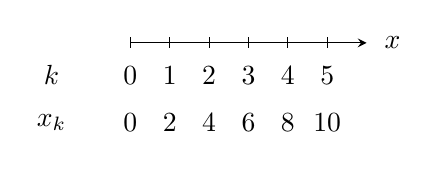
\begin{tikzpicture}[
        ]
        % draw horizontal line   
        \draw[myptr] (0,0) -- (3,0) node[right=3pt] {$x$};
        
        % draw vertical lines
        \foreach \k/\xk in {0/0, 1/2, 2/4, 3/6, 4/8, 5/10}
        {
            \draw (\k*0.5 cm,2pt) -- (\k*0.5 cm,-2pt)  node[below=3pt] (k\k) {$\k$} node[below=20pt] (xk\k) {$\xk$};
        }
        \node[left of=k0] {$k$};
        \node[left of=xk0] {$x_k$};
        % draw nodes
    \end{tikzpicture}

    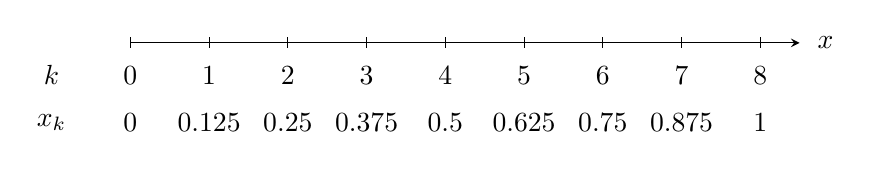
\begin{tikzpicture}[
        ]
        % draw horizontal line   
        \draw[myptr] (0,0) -- (8.5,0) node[right=3pt] {$x$};
        
        % draw vertical lines
        \foreach \k/\xk in {0/0, 1/0.125, 2/0.25, 3/0.375, 4/0.5, 5/0.625, 6/0.75, 7/0.875, 8/1}
        {
            \draw (\k cm,2pt) -- (\k cm,-2pt)  node[below=3pt] (k\k) {$\k$} node[below=20pt] (xk\k) {$\xk$};
        }
        \node[left of=k0] {$k$};
        \node[left of=xk0] {$x_k$};
        % draw nodes
    \end{tikzpicture}



    sss

	\begin{minipage}[t]{0.09\textwidth}
        $x_1$
	\end{minipage}
	\begin{minipage}[t]{0.91\textwidth}
        \begin{align*}
            \gpp[\widetilde{T}][2][2^2][x_1][x_1][x_1] & \\
            \gpp[\widetilde{T}][][2^2][x_2][x_1][x_0] & \\
            \gppn[T_2][T_1][T_0][2^2] & \\
            \gppn[40][T_1][T_0][2^2] &
        \end{align*}
	\end{minipage}

    
    \begin{tabular}{lll}
        \text{{\color{blue}\uline{Hyperpolic}}} & & \text{{\color{red}\uline{Parabolic}}} \\
        $ {\color{blue}r = \f{\dt}{\dx}} $      & ${\color{red}\neq}$ & ${\color{red}r = \f{\dt}{\dx[2]}}$
    \end{tabular}

    

    

    $ \Delta u=u_{xx}+u_{yy}=0 $

    $\Delta u=u_{xx}+u_{yy}=f(x,y)$

    $ \Delta u =  u_{xx} + u_{yy} = \frac{\partial^2 u}{\partial x^2} + \frac{\partial^2 u}{\partial y^2} = 0 $

    \begin{tabular}{ll}
        Nabla Operator                  & $\nabla{u} = u_{x}+u_{y} = \frac{\partial u}{\partial x} + \frac{\partial u}{\partial y}$ \\
        Laplace Operator                & $\Delta{u} = u_{xx} + u_{yy} = \frac{\partial^2 u}{\partial x^2} + \frac{\partial^2 u}{\partial y^2} $\\
        \hline
        \hline
        Anfangswertproblem (AWP)        & \multirow{2}{*}{$u\kl{x,0} = f\kl{x}, \quad {\textstyle\f{\partial u}{\partial x}}\kl{x,0} = g\kl{x}$} \\
        Initial value problem (IVP)     & \\
        \hline
        Randwertproblem (RWP)           & \multirow{2}{*}{$u\kl{x,a} = \alpha, \quad u\kl{x,b} = \beta $} \\
        Boundary value problem (BVP)    & \\
        \hline
        Dirichlet-Randbedingung         & $u\kl{x,0} = f\kl{x}$ \\
        Dirichlet boundary condition    & Werte auf dem Rand liegend \\
        \hline
        Neumann-Randbedingung           & ${\textstyle\f{\partial u}{\partial x}}\kl{x,0} = f\kl{x}$ \\
        Neumann boundary condition      & Ableitungswerte auf dem Rand liegend \\
        \hline
        Laplace-Gleichung               & \multirow{2}{*}{$\Delta u = 0 $}\\
        Laplace's equation              & \\
        \hline
        Poisson-Gleichung               & \multirow{2}{*}{$-\Delta u = f $}\\
        Poisson's equation              &
    \end{tabular}

    \begin{tabular}{lll}
        \multicolumn{3}{c}{$ Au_{xx} + 2Bu_{xy} + Cu_{yy} + Du_x + Eu_y + Fu +G= 0 $} \\
        \hline
        Elliptische PDF                 & Laplace-/Poisson-Gleichung    & \multirow{2}{*}{$ B^2 - AC < 0$} \\
        Elliptic PDE                    & Laplace-/Poisson's equation   & \\
        \hline
        Parabolische PDF                & Wärmeleitungsgleichung, Diffusionsgleichung         & \multirow{2}{*}{$ B^2 - AC = 0$} \\
        Parabolic PDE                   & Heat equation, Diffusion equation                 & \\
        \hline
        Hyperbolische PDF               & Wellengleichung               & \multirow{2}{*}{$ B^2 - AC < 0 $} \\
        Hyperbolic PDE                  & Wave equation                 &
    \end{tabular}

    \subsection*{Finite Difference Method (FDM)}
    \subsection*{Elliptic PDEs}
    \subsubsection*{Dirichlet Boundary Conditions}
    
    Discrete Laplace-Operator

    \begin{align*}
        \Delta u & = u_{xx} + u_{yy} \\
        h        & = \dx = \dy \\
        \Delta u & \approx \f{1}{h^2} \kq{u\kl{x + h, y} + u\kl{x, y + h} + u\kl{x - h, y} + u\kl{x, y - h} - 4 \cdot u\kl{x,y}} \\
        \Delta u & \approx \f{1}{h^2} \kq{u\kl{P_E} + u\kl{P_N} + u\kl{P_W} + u\kl{P_S} - 4 \cdot u\kl{P_C}}
    \end{align*}

    \subsubsection*{Neumann Boundary Conditions}

    \begin{align*}
        u_x\kl{P_C} & \approx \f{u\kl{P_E} - u\kl{P_W}}{2\cdot h} \\
        u\kl{P_W}   & = u\kl{P_E} - 2\cdot h \cdot u_x\kl{P_C} \\
        \Delta u    & \approx \f{1}{h^2} \kq{u\kl{P_E} + u\kl{P_N} + {\color{red}u\kl{P_W}} + u\kl{P_S} - 4 \cdot u\kl{P_C}} \\
                    & \approx \f{1}{h^2} \kq{u\kl{P_E} + u\kl{P_N} + {\color{red}u\kl{P_E} - 2\cdot h \cdot u_x\kl{P_C}} + u\kl{P_S} - 4 \cdot u\kl{P_C}} \\
                    & \approx \f{1}{h^2} \kq{{\color{red}2\cdot}u\kl{P_E} + u\kl{P_N} + u\kl{P_S} - 4 \cdot u\kl{P_C} {\color{red} - 2\cdot h \cdot u_x\kl{P_C}}} \\
    \end{align*}
    
    \subsection*{Parabolic PDEs}
    \subsubsection*{Richardson's Explicit Method}
    
    \begin{align*}
        u_{t}\kl{x,t}                               & = u_{xx}\kl{x,t} \\
        \f{u \kl{x, t + \dt} - u \kl{x, t}}{\dt}    & = \f{u \kl{x + \dx, t} - 2 \cdot u\kl{x, t} + u \kl{x - \dx, t}}{\dx[2]} \\
        r                                           & = \f{\dt}{\dx[2]} \\
        u \kl{x, t + \dt}                           & = r \cdot \kq{u \kl{x + \dx, t} - 2 \cdot u\kl{x, t} + u \kl{x - \dx, t}} - u \kl{x, t} \\
        u_{x,t+1}                                   & = r \cdot \kq{u_{x+1,t} - 2 \cdot u_{x,t} + u_{x-1,t}} - u_{x, t} \\
        u_{x,t+1}                                   & = r \cdot u_{x-1,t} + \kl{1 - 2\cdot r} \cdot u_{x,t} + u_{x+1,t} \\
        u_{\dt + 1} & = \ks{\ldots}  u_{\dt}
    \end{align*}

\end{document}
